\documentclass{article}

\usepackage[inline]{enumitem}

\usepackage{url}
\usepackage{graphicx}
\graphicspath{ {./figures/} }
\usepackage{amsfonts}% to get the \mathbb alphabet
\usepackage{booktabs}
\usepackage{multirow}


\title{Decentralised Mining Pool for Bitcoin (Draft 0.1)}
\author{}
\date{}

\begin{document}

\maketitle

\begin{abstract}
  Bitcoin p2pool's usage has steadily declined over the years,
  negatively impacting bitcoin's decentralisation. The primary
  problems with p2pool are twofold. First, the variance in earnings
  for miners increases with total hashrate participating in the
  pool. Second, payouts to miners require a linearly increasing
  blockspace with the number of miners participating in the
  pool. There are two different proposals under discussion that
  address these problems,
  \begin{enumerate*}[label=(\roman*)]
  \item building a directed acyclic graph (DAG) of miner's shares such
    that miners are rewarded for all their proof of work, and
  \item  using payment channels to distribute payouts to miners
  \end{enumerate*}. In this paper, we present a solution that builds
  on these two proposals. A DAG of shares is maintained as a
  replicated database by all miners and the DAG is then used to
  compute rewards for miners. These mining rewards are paid out by an
  anonymous hub communicating with the miners using I2P. Using the
  payment channels construction, neither the hub nor the miners can
  cheat. We show that our approach is incentives compatible and
  describe how the hub maintains its anonymity to resist DDoS attacks.
\end{abstract}
   
\section{Motivation}

P2Pool~\cite{p2pool:wiki} helps bitcoin's decentralisation by allowing
miners to select the transactions they mine. This avoids any potential
transaction censorship by pool operators. However, the construction
used by P2Pool faces a number of problems that has resulted in miners
abandoning the pool. The most often cited problems are:

\begin{enumerate}
\item large variance in earnings for miners,
\item large number of stale blocks, and
\item large block space requirement for payouts.
\end{enumerate}

The first two problems are a direct consequence of the shares block
rate limited to 30 seconds on the bitcoin p2pool. Intuitively, as the
hash rate participation in the pool goes up, the difficulty for 30
seconds block rate goes up and smaller miners find it harder to find
shares within a 30 second period. This results in an increase in the
variance for shares found by miners and thus for the rewards earned by
the miners. Ethereum's inclusive protocols~\cite{inclusive-protocols}
address the problem by building a DAG of blocks and rewarding blocks
that otherwise would have been left out as stale blocks. As miners get
rewarded for more of their work, the variance on their earnings
reduces enabling smaller miners to remain economically viable.

Payouts in P2Pool are included in the coinbase of the block being
mined. As the number of participants in P2Pool increase the size of
the coinbase transaction increases taking up valuable blockspace that
the miners could have earned fees from instead. This imposes an
upper bound on the number of participants in P2Pool.

Knowing the challenges faced by P2Pool, we list the goals of a new
decentralised mining pool as:

\begin{enumerate}
\item Reduce variance for miners with increasing pool hash rate.
\item Make payouts to miners with constant size block space
  requirement.
\item Allow miners to select transactions they want to mine, with no
  potential for a censor to deny payouts.
\item Provide building blocks for a hash rate futures
  market.~\footnote{We don't elaborate on this goal in this paper, but
    readers can look up the gist on TerraHash coins
    https://gist.github.com/kulpreet/19927c7188a4224ce2de43efb3c69370}
\end{enumerate}

\section{Current Proposals}

TerraHash Coin~\cite{mcelrath:variance}, Jute~\cite{jute} and
Spectre~\cite{spectre} use a DAG for faster block times and focus on
changing the consensus layer of bitcoin. These proposals allow for
miners to produce shares that include conflicting transactions and
then apply rules to find a set of transactions acceptable at various
cuts of the DAG, such that the bitcoin consensus rules are not
violated.

Braiding the blockchain proposal~\cite{mcelrath:variance} shows how,
smaller more frequent blocks can form a DAG of blocks, called a braid,
with each block pointing to one or more one previous blocks. Blocks in
the braid are called beads and can have transactions repeated in
different blocks. The proposal describes how duplicate and double
spend transactions can be resolved to reach a decision on the state of
the ledger at any cut of the DAG.\@

In the proposal, miners earn a coin native to the braid blockchain,
called TerraHash Coin. This coin can then be swapped for BTC. The
proposal doesn't yet define how this native coin will be swapped for
bitcoin. Some of the suggestions under discussion include using atomic
swaps, burning the TerraHash Coin, or using financial instruments like
futures of the bitcoin's hash rate to swap TerraHash Coins for BTC.\
The problems with the atomic swap approach is the need for $O(n)$
block space in number of miners, as we need two transactions to
execute a swap with each miner payout. Burning THCoins for BTC
requires a trusted third party to execute the burn. Finally, trading
THCoins for BTC futures has the problem of introducing centralisation
on the futures market operator. There is some discussion around using
DEXes for executing futures contracts, but these are initial ideas and
we will evaluated them in the future for incorporating them into our
proposal once they have been developed further.

Belcher~\cite{channels-for-rewards} proposes using payment channels to
avoid using block space for making payouts to miners. The construction
uses payment channels between federated hubs to pay miners after a
block has been successfully mined. The payouts are made after a long
period, similar to the 100 blocks requirements for spending from
coinbase transactions. The hub locks in BTC for each miner by opening
payment channels for each of the miners. The construction shows how
both miners and the hub can not cheat and how the funders of the hub
earns rewards for funding the payment channels.

The two ideas of using a DAG and payment channels for rewards
payouts together present a potential path for rebooting P2Pool. In the
rest of the paper we present a modified version of TerraHash Coin and
show how the various components work together.

\section{Decentralised Bitcoin Mining}

In this section we present a modified version of TerraHash Coin. We
propose building a DAG of miner's shares and use that to determine the
payout distribution between miners. We then show that miners are
rewarded for shares that they broadcast to the p2p network in a timely
manner.

\subsection{A DAG of Shares}

\begin{figure}
  \begin{center}
    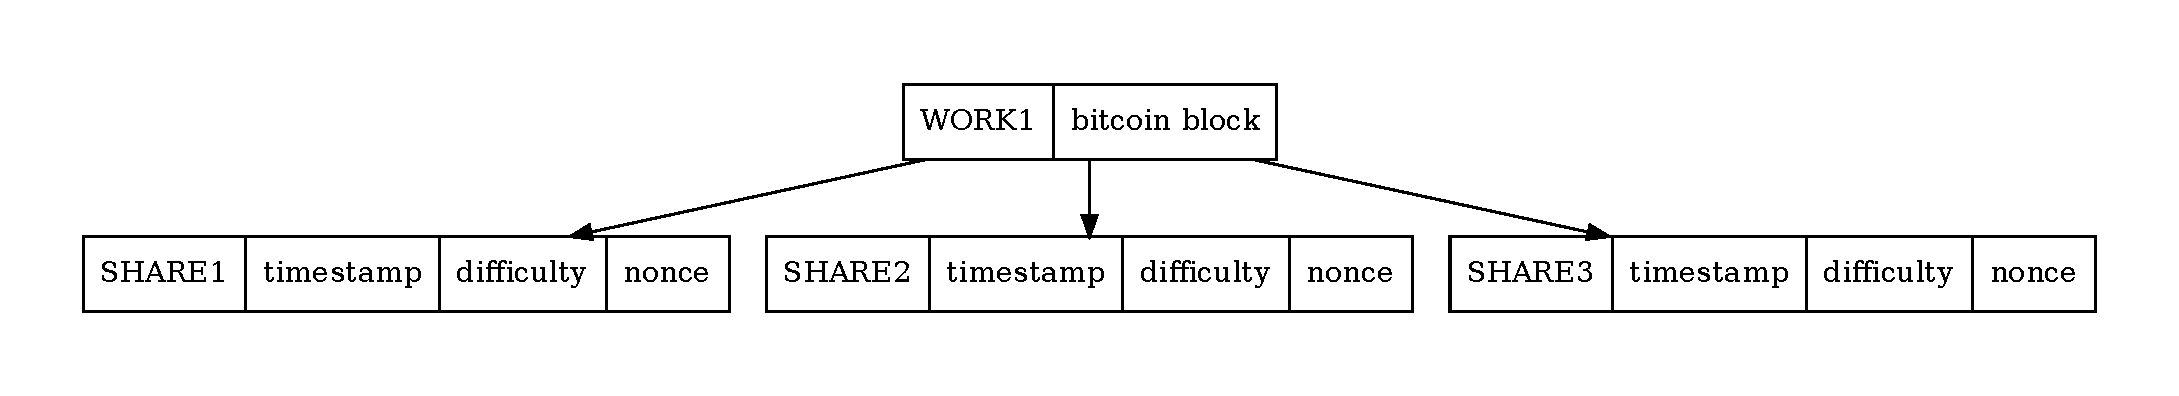
\includegraphics[width=1\textwidth]{work-share}
    \caption{Each \textsc{work} generated and shared by a miner is then
      followed by the \textsc{share}s the miner finds.}\label{fig:work-share}
    \end{center}
\end{figure}

Each miner builds their own block, selecting transactions according to
their own criteria. We call this block the \textsc{work} and it is
derived from the results of the \verb|getblocktemplate| bitcoin API
call. The \textsc{work} definition leaves out the merkle root,
timestamp and the difficulty. Instead it includes the coinbase
transaction so that other pool participants can verify that the
\textsc{work} definition includes the correct payout
scripts. Table~\ref{table:work} shows the \textsc{work} built by
miners and then broadcast to the entire p2p network. The transactions
field is compressed using the same techniques as specified in the
compact block specifications~\cite{compact-blocks}.

\begin{table}
  \centering
  \begin{tabular}{ |l|p{0.4\linewidth}|r| }
    \hline
    \multicolumn{3}{|c|}{\textsc{work}} \\
    \hline
    Field & Description & Size in bytes \\
    \hline
    Version & Bitcoin block's version field & 4\\
    \hline
    Previous block & Hash of the previous bitcoin block & 32 \\
    \hline
    Coinbase & Coinbase for payment channel setup, see Section~\ref{ref:channels} & 38 \\
    \hline
    Transactions & Transaction ids included in the block & variable \\
    \hline
    \textsc{Work} hash & Hash of the above fields & 32 \\
    \hline
  \end{tabular}
  \caption{The structure of \textsc{work} broadcast by
    miners. Timestamp, difficult and nonce are left for the
    \textsc{share} to specify }\label{table:work}
\end{table}

The miner then starts mining on \textsc{work} and generates
\textsc{share}s. Figure~\ref{fig:work-share} shows the relationship
between \textsc{work} and its \textsc{share}s. Each \textsc{work}
created by a miner can result in multiple \textsc{share}s and both the
\textsc{work} and \textsc{share}s are broadcast to the p2p
network. When a miner receives a \textsc{work} from other miners it
validates this \textsc{work} using a local bitcoin node. When a
\textsc{share} is received by a miner it is validated against the
\textsc{work} referenced by the \textsc{share}.

\begin{table}
  \centering
  \begin{tabular}{ |l|p{0.4\linewidth}|r| }
    \hline
    \multicolumn{3}{|c|}{\textsc{Share}} \\
    \hline
    Field & Description & Size in bytes \\
    \hline
    \textsc{Work} hash & Hash used to identify the \textsc{work} for this share & 32 \\
    \hline
    Nonce and extra nonce & Nonces used & $4+8$ \\
    \hline
    Merkle root & New merkle root to include extra nonce & 32 \\
    \hline
    Timestamp & UNIX timestamp used & 4 \\
    \hline
    Difficulty & Claimed difficulty miner is using, if different from last share. & 4 \\
    \hline
    Public keys & Two pubkeys used by the hub to for channel management & 66 \\
    \hline
    $list<$ \textsc{share} hashes $>$ & List of share hashes referenced by this \textsc{share} & $N \times 32$ \\
    \hline
    I2P destination & The I2P destination for hub-miner communication, see Section~\ref{sec:hub-miner-communication}. & 387 \\
    \hline
    Total size & \multicolumn{2}{|r|}{$505 + N \times 32$} \\
    \hline
  \end{tabular}
  \caption{The structure of \textsc{share}s broadcast by miners. Size
    of the \textsc{share} is dependent on the size of the
    network.}\label{table:share}
\end{table}


Table~\ref{table:share} shows the structure of \textsc{share}s
broadcast by the miner. Each \textsc{share} includes the hash of the
\textsc{work} the miner is working on, along with the current target
difficulty used by the miner, the public keys that the hub uses to
setup payment channels, and finally an I2P destination address of the
miner.

Miners broadcast their \textsc{share}s to the network using a gossip
protocol and all the miners maintain the DAG of \textsc{share}s as a
replicated database. Each node on the DAG is a \textsc{share}
generated by a miner and all miners track the most recently received
\textsc{share} from all other miners. Miners include a hash pointer to
the most recent known \textsc{share}s from all miners in its own
\textsc{share}. This leads to all edges in the DAG pointing from a
\textsc{share} to all the \textsc{share}s known by the miner when
starting to mine a \textsc{work}. This construction of the DAG ensures
that the DAG is eventually consistent on all p2p participants. The DAG
also includes valid bitcoin blocks, since one of the shares eventually
satisfies the then bitcoin difficulty requirement. The downside is the
that the size of \textsc{share} will increase linearly with the size
of the network and will lead to an upper bound on the size of the
pool. With $N = 10,000$, the size of the share is $320kB$, which is
small enough for fast propagation across a $10,000$ node peer to peer
network~\cite{information-propagation}. However, scaling by another
order of magnitude will require optimisations to the \textsc{share}
structure.

\begin{figure}
  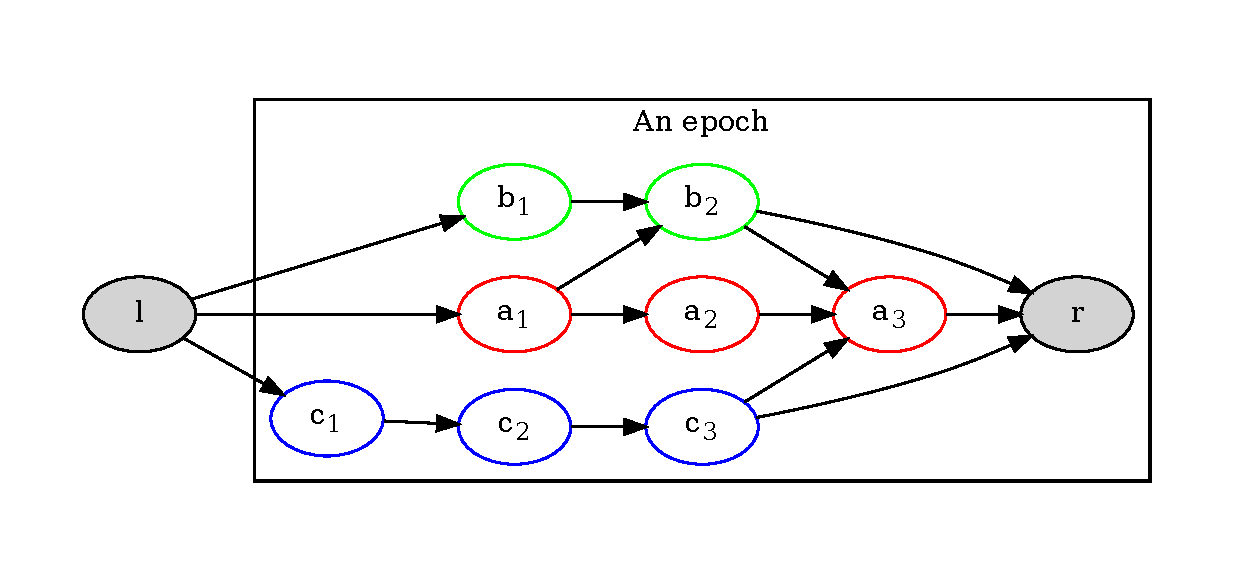
\includegraphics[width=1.0\textwidth]{epoch}
  \caption{A epoch is defined as all the \textsc{share}s mined between two
    bitcoin blocks. Here all the \textsc{share}s between $l$ and $r$ are in
    the same $epoch$.}\label{fig:epoch}
\end{figure}

Each \textsc{share} that matches or exceeds the current bitcoin
difficulty starts a new $epoch$ for the p2p mining
pool. Figure~\ref{fig:epoch} shows a DAG with three miners
participating in the pool, $a$, $b$ and $c$. The nodes in the DAG are
the shares generated by the three miners. Nodes $l$ and $r$ are two
valid bitcoin blocks that have been mined such that they meet
bitcoin's difficulty at the time, and all the blocks between $l$ and
$r$ are in the same $epoch$. All shares in an epoch have a path from
$l$ to itself and a path from itself to $r$. Any shares that don't
have a path from $l$ and to $r$ are not considered to be part of the
$epoch$.

\subsubsection{Miner Defined Difficulty}\label{sec:share-difficulty}

The nodes in the DAG are \textsc{share}s mined at difficulty level
selected by the miner. This difficulty can be dynamically changed by
the miner after each \textsc{share}, depending on the miner's
observation of the p2p network's hashrate. This dynamic difficulty
adjustment allows miners to adjust the rate at which they produce
\textsc{share}s. This is important as smaller miners can produce low
difficulty shares to match the share rate of the larger miners in the
pool. Even if smaller miners earn a smaller reward, they will earn
these rewards for all their work.

In the next section we then describe how all peers compute their fair
share of profits using the DAG of shares. We then show how our reward
computation algorithm is incentives
compatible~\cite{incentives-compatible}.

%% - block datastructure
%%   - coinbase reward goes to Hub's address
%%   - ignore this for now, we'll show how the reward is distributed in a
%%     trustless manner to all miners.
%% - DAG of shares
%%   - Epochs: start from and end with bitcoin block
%%   - Epoch ends when a valid bitcoin block with current bitcoin
%%     difficulty is found
%%   - Immediately send mined bitcoin block to bitcoin network
%%   - Hub will distribute the reward in around 100 blocks time
%% - Use compact blocks to inform others about the block we are mining
%%   - Other miners can decide to include your block as a previous block
%%     or not, whenever we find a solution and announce it.
%%   - We need to model the network traffic and latency
%% - Keep mining the same block, until end of epoch
%%   - For each block mined, share the solution with p2p network
%%   - Only if the mined block meets the current bitcoin difficulty
  
  
\subsection{Incentives Compatible Rewards}\label{sec:rewards}

Each participating node, which includes the miners and the hub,
maintains a local replica of the the \textsc{share}s DAG.\@ Each
\textsc{share} includes a reference to the shares the miner was aware
of when the \textsc{share} was found. If a miner $a$ doesn't include
the \textsc{share}s of miner $b$, it signals a failure of
communication between the two miners. We introduce a rule that miner
$a$ in such a situation stops including references to $b$'s
\textsc{share}s.

The incentive in lay terms is that all miners should include the
\textsc{share}s discovered by other miners, as otherwise they will be
excluded by other miners and they will lose the opportunity to be
rewarded for their work. We identify a degenerative case as ``isolated
miners'' and argue that miners have no incentives to act in this
manner. Figure~\ref{fig:isolated-miners} shows a DAG where all three
miners $a$, $b$ and $c$ are working independently. In such a situation
when the miner $a$ discovers a share $a_3$ that is a valid bitcoin
block the reward is not shared with any other miner as $a_3$ does not
include any references to shares from other miners.

\begin{figure}
  \begin{center}
    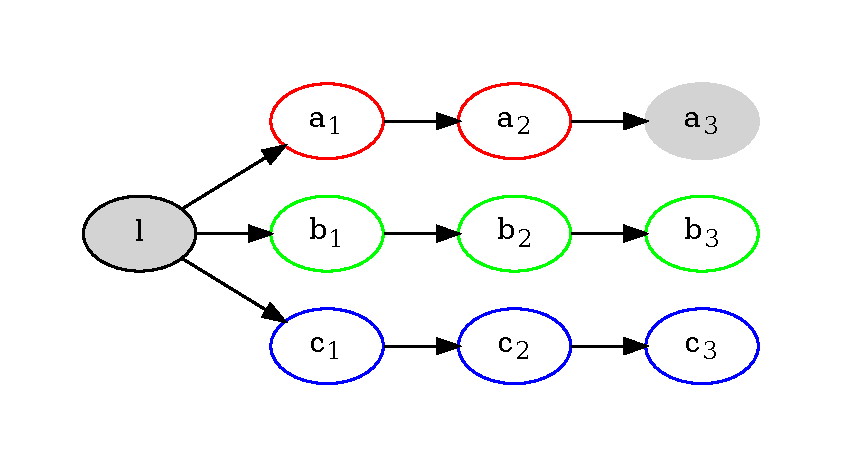
\includegraphics[width=0.65\textwidth]{isolated-miners}
    \caption{$a$ discovers a share and the reward is not shared with any
      other miner.}\label{fig:isolated-miners}
  \end{center}    
\end{figure}

With the above understanding of why miners will co-operate, we now
state the rules to calculate how the block reward should be divided
between miners.

\begin{enumerate}
\item Traverse the DAG in reverse order from the \textsc{share} that
  found a bitcoin block to the previous bitcoin block found and
  collect this set of shares.
\item From the above set of shares remove all shares that don't have
  a reverse path to the previous bitcoin block.
\item Distribute the reward between miners weighted by the sum of
  the difficultly of all \textsc{share}s found by miners.
\end{enumerate}

As an example, consider the p2p network of miners $a$, $b$ and $c$
with the DAG of shares as shown in Figure~\ref{fig:shares-dag}. In the
DAG, the set of shares that receive reward proportional to their
difficulty are $\{a_1..a_5, b_1..b_3\}$. The shares $\{c_1..c_3\}$ do
not receive any reward as they are not reachable from the bitcoin
block, $a_5$, even if they are reachable from $l$. In other words,
since the shares $\{c_1..c_3\}$ are not part of the $epoch$
terminating in $a_5$ the miner $c$ is not rewarded for those
shares. We exclude the shares $c_1..c_4$ from the set of shares to be
rewarded to avoid miners indulging in selfish
mining~\cite{majority-is-not-enough}.

For the second bitcoin block $b_5$ only the miners $a$ and $b$ receive
rewards in proportion to the difficulties of their shares
$\{b_4, b_5, a_6\}$. $c$ doesn't receive any reward for $c_4$ as it
again is not part of the $epoch$ terminating in $c_5$.

\begin{figure}
  \begin{center}
    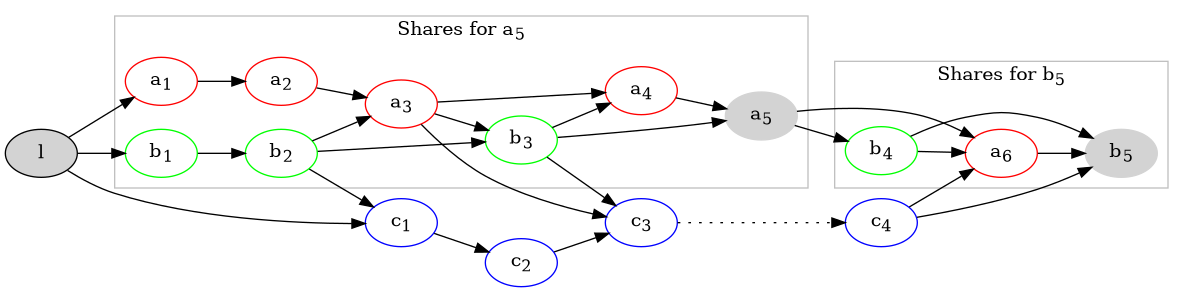
\includegraphics[width=1.0\textwidth]{shares-dag}
    \caption{Two epochs in a DAG of shares mined by three mines ---
      $a$, $b$ and $c$. The shares in grey meet the bitcoin difficulty
      at the time they were mined.}\label{fig:shares-dag}
  \end{center}
\end{figure}

Given the above rules, we show how they together provide an incentives
compatible reward function~\cite{incentives-compatible}. We present an
outline of proofs that will be be formalised in future work.

\subsubsection{Incentive Compatibility}\label{sec:incentive-compatability}

A reward function is defined as incentive compatible if every miner's
best response strategy reports full solutions
immediately~\cite{incentives-compatible}. Where a ``full solution'' is
a share that meets the bitcoin network's difficulty requirement.

Given the rules in Section~\ref{sec:rewards}, if a miner finds a
bitcoin block the miner wants to get maximum reward possible based on
all the shares it has found and therefore is incentivized to announce
their \textsc{share} as soon as it finds the block. The longer a miner
waits to announce the bitcoin block to the bitcoin network, the higher
the probability that some other miner on the pool will find a
different bitcoin block that doesn't reward their latest shares that
haven't reached the other miner. Further still, the rewards
calculation can be adjusted to give an extra reward to the miner that
finds the block. This is similar to what p2pool does and Belcher also
mentions in his proposal.

\subsubsection{Proportional Payments}\label{sec:proportional-payments}

Proportional payments~\cite{incentives-compatible} property requires
that the pool pays miners in proportion to the amount of work they
have performed. According to our rewards calculation rules, payouts
are calculated at the end of an epoch and each miner is incentivized
to include hash pointers to the most recent shares seen from all
miners. It directly follows that all miners are guaranteed payments
for their shares that have reached the miner who found the
block. Therefore the pool satisfies this requirement.

\subsubsection{Budget Balanced}\label{sec:budget-balanced}

Budget balanced~\cite{incentives-compatible} property requires that
pool operator to never incur a deficit. Again from the rules above,
since rewards are paid at the end of the epoch, a hub pays out rewards
without losing or retaining any amount. The hub therefore does not
make an unaccounted for profit or loss.

\subsection{Lost Work or Stale Shares}\label{ref:stales}

\begin{figure}
  \begin{center}
    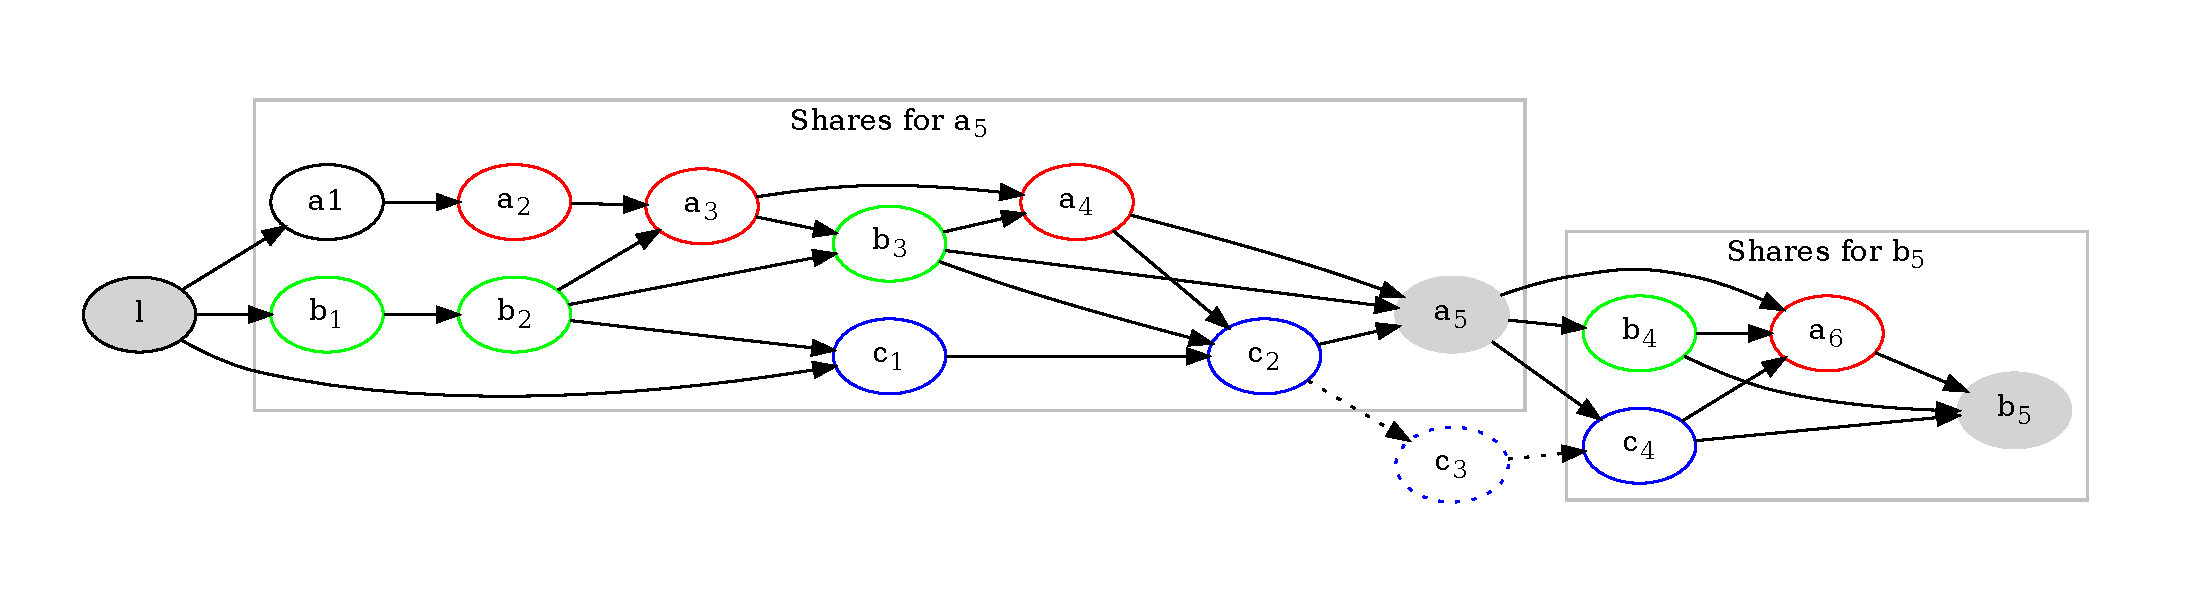
\includegraphics[width=1\textwidth]{shares-propagation.pdf}
    \caption{Share $c_3$ is a stale share that $c$ earns no reward
      for.}\label{fig:shares-propagation}
  \end{center}
\end{figure}

We define a share to be stale share if it is not included in two
consecutive epochs. In Figure~\ref{fig:shares-propagation} the share
$c_3$ is a stale share as it is not included in the $epoch$s
terminating in either $a_5$ or $b_5$. We don't reward miners for these
stale shares as that allows miners to indulge in selfish
mining~\cite{majority-is-not-enough}. In this section we show some
very rough estimates on the work lost by the miners for not being
reward for these stale shares.

The details of the p2p network to transmit shares is not yet
specified, and we don't have simulations results to observe the impact
of the the pool size both in terms of number of miners and the total
hash rate of the pool. For now, we present a high level analysis of
the work lost from stale shares.

Say $t_{s}$ is the time in seconds to transmit a share to all other
participants in the network.  Let $t_{b}$ be the time it takes for the
pool to find a block. It follows that, in the worst case, each miner
will waste $t_{s}/t_{b}$ amount of work for the time when its work
fails to reach the miner who finds the next block.

We work with estimates from observations about block transmission on
the bitcoin p2p network~\cite{information-propagation} but keep in
mind caveats that the observations there include the time to verify
the block and that \textsc{work} size at $320kB$ for a p2p network
with $N = 10,000$ is much smaller than a bitcoin block.

Given the caveats We proceed to use the same propagation delays from
the study to capture upper bounds of the work lost and assume a $10$
second delay for a \textsc{share} to reach all other nodes on the p2p
network. We also assume that $10,000$ miners pool reaches $2\%$ of the
global hashrate. This is similar to $12,000$ miners achieving $2\%$
hashrate by Slushpool~\cite{slushpool}. With this assumption we can
say that the pool finds a block every $50$ blocks, or approximately
every $500$ minutes.

From the above, we get $t_{s} = 10$s and $t_{b} = 500$ minutes and get
the lost work of around $0.03\%$. Adding the $0.1\%$ fees the miners
pay to the hub, the miners end up paying $0.13\%$ in costs as compared
to $2\%$ on mining pools, which is still a saving of around $93\%$ in
fees for the miner when using a decentralised pool.


% From early studies on information dissemination using gossip protocol
% it is known that with $5$ retransmissions of a payload, we can reach
% $99.88\%$ of nodes for a 1000 node
% network\cite{epidemic-algorithms}. Making some pessimisitc assumptions
% here to find out the upper bounds on the work lost. If all the $5$
% transmissions are to far away miners, with a latency of $400ms$, then
% a share will be distributed to $99.9999\%$ of nodes within a $2s$
% interval.

\subsection{Payment Channels}\label{ref:channels}

We propose using Payment Channels for paying miners based on the
proposal by Belcher~\cite{channels-for-rewards}. The construction of
the payments channels we present is similar to Belcher's construction,
but there are a few changes and we highlight them before describing
the details.

\begin{itemize}
\item In the Belcher proposal, the pool had to predict how much work
  miners will be able to contribute for the next block. Instead our
  DAG based scheme results in an incentives compatible distribution of
  rewards among miners.
\item Belcher proposes uses multiple hubs to prevent DDoS attacks on
  hubs, we instead use a single hub, and prevent DDoS attacks by
  keeping the hub hidden using I2P~\cite{i2p,
    i2p-censorship-resistance} for communication between the hub and
  miners.
\end{itemize}

The rest of the construction is similar to the early versions
presented by Belcher --- there is a one-way channel between the hub
and each of the miners. The hub updates the state of each channel with
appropriate reward after each block is found.

% TODO
% Question: How do we know the Hub is not creating coinbases with
% different preimages with each miner?

% Answer: Miners receive the pubkey for all other miners with the
% \textsc{work} announcement. Using this and the structure of the
% coinbase transactions, miners validate that the coinbase matches the
% hub's preimage, and the miner's pubkey.

\subsubsection{Coinbase}

We use Belcher~\cite{channels-for-rewards} construction where each
miner builds a coinbase transaction that can be spent in one of the
following three ways:

\begin{enumerate}
\item Co-operatively by Hub and Miner, or
\item By the Hub with a hash lock for pre-image \verb|X|, or
\item By the Miner that found the bitcoin block, but after waiting for
  six months.
\end{enumerate}

\begin{table}
  \centering
  \begin{tabular}{ lr }
    \bfseries Coinbase \\
    \midrule
    \verb|2 H M 2 CHECKMULTISIG| & $(cb_1)$ \\
    \verb|OR| \\
    \verb|hash(X) + Hub P2WPKH| & $(cb_2)$ \\
    \verb|OR| \\
    \verb|M and CHECKSEQUENCEVERIFY 6 months| & $(cb_3)$\\ 
    \midrule
  \end{tabular}
  \caption{Coinbase transaction with hub and miner public keys.}\label{table:coinbase}
\end{table}

The scriptPubKey for the above conditions in the coinbase is shown in
Table~\ref{table:coinbase}. These conditions mean that the hub can not
spend the coinbase without revealing the pre-image $X$. This pre-image
is included in the construction of payment channels, as we will see in
the next section. This use of pre-image in both the coinbase and the
payment channel definition guarantees that miners get paid for their
accumulated payouts if the Hub defects and spends through the $cb_2$
branch. We discuss how the miner and the hub don't gain by defecting
in Section~\ref{ref:defecting}.

\subsubsection{One-way Channels}

One-Way payment channels between hub and all miners allow miners to
receive payouts while consuming a constant size blockspace in the
bitcoin block they mine. The use of payment channels is what makes the
pool scale without losing blockspace. The miners therefore avoid
losing the fees that can be earned from the blockspace.

Just like in the early versions of proposal by Belcher we use one-way
payment channels. One-Way payment channels solve the problem of
aggregating a miner's payouts requiring a single blockchain
transaction for spending multiple payouts earned from their PoW
shares.

We use one-way instead of bidirectional payment channels as an initial
implementation. If required we can switch to bidirectional
channels~\cite{poon2016bitcoin} allowing miners to spend their mining
payouts over the lightning network. However, for now, we deliberately
stay away from the complexity of making the hub a lightning node. If
there is interest from miners to use the lightning network, we can
build it in the future.

Each miner has a one-way payment channel with the hub using a two of
two multisig with a time lock of six months. For each payout a miner
receives over the payment channel, the hub will charge an agreed upon
fees between the miner and the hub. Belcher's proposal recommends a
$0.1\%$ fees for the hub.

\subsubsection{Payment Channel Transactions}

The hub creates a funding channel locking an amount $R$ of
bitcoin. The miner then creates a refund transaction, spending the
funding transaction and sending the $R$ bitcoin back to the hub. The
refund transaction has a locktime of six months allowing the miner to
accumulate their payout over the six month period. The protocol can be
extended to allow each miner to agree upon a locktime with the hub. In
this case, the trade-off will be between the fees charged by the hub
and the length of the locktime.

The funding transaction includes an input from the hub and an output
that can be spent in one of the two conditions shown in
Table~\ref{fund-tx}. \verb|H| and \verb|M| are the public keys for hub
and miner, they are called the co-operative keys by Belcher. While
\verb|H'| and \verb|M'| are alternative public keys for hub and miner,
and are called the uncooperative keys in the Belcher proposal.


\begin{table}
  \centering
  \begin{tabular}{ llr }
    \multicolumn{2}{c}{\bfseries Fund Transaction} \\
    \midrule
    \bfseries Input & \bfseries Output \\
    \midrule
    Hub's UTXO & \verb|2 H  M  2 CHECKMULTISIG| & $(f_1)$ \\
    (Signed by the hub) & \verb|OR| \\
                    & \verb|2 H' M' 2 CHECKMULTISIG + Hash(X)| & $(f_2)$ \\
    & (R coins) \\
    \midrule
  \end{tabular}
  \caption{Fund transaction for payment channel between hub and miner.}\label{fund-tx}
\end{table}


The hub doesn't broadcast the funding transaction, instead it waits
for the miner to create refund transaction. This is the same as any
other timelocked one-way channel construction, i.e.\ the miner creates
a refund transaction with a timelock, signs it and sends it to the
hub. The refund transaction is shown in Table~\ref{refund-tx}.

\begin{table}
  \centering
  \begin{tabular}{ ll }
    \multicolumn{2}{c}{\bfseries Refund Transaction. Locktime 6 months} \\
    \midrule
    \bfseries Input & \bfseries Output \\
    \midrule
    Fund Tx & \verb|P2WPKH Hub's address| \\
    (Signed by miner) & (R coins) \\
    \midrule
  \end{tabular}
  \caption{Refund transaction signed by miner and held by
    hub.}\label{refund-tx}
\end{table}

With the refund transaction, if the miner stops responding, the hub
can get a refund in six months time. However, the hub can be attacked
by sending requests to open new channels and locking up the hub's
liquidity. We resolve this by requiring the hub to open a channel to a
miner only after it has contributed enough shares. This can be a
parameter of the pool instantiation, with values anywhere between one
to 100 bitcoin blocks. The threshold number of shares required before
opening the channel is a configuration parameter for the hub. The
miner will still receive the payouts for the shares generated, it is
only that the channel opening is delayed.

On receiving the refund transaction, the hub broadcasts the funding
transaction. Once the funding transaction is confirmed, the hub can
start sending payouts to the miner. These payouts are determined in
proportion to the shares found by the miner and included in the DAG as
described in Section~\ref{sec:rewards}.

The payment transactions are updates to the channel where each update
increases the earnings of the miner. The payment transactions are
signed by the hub using the non-cooperating key, \verb|H'|.
Table~\ref{payment-transaction} shows the structure of the payment
transactions. In the next section we present how the payouts are
distributed, we then show how the hub and the miners are
dis-incentivized to cheat.


\begin{table}
  \centering
  \begin{tabular}{ llr }
    \multicolumn{2}{c}{\bfseries Payment Transaction} \\
    \midrule
    \bfseries Input & \bfseries Output \\
    \midrule
    Fund Tx & \verb|2 H  M  2 CHECKMULTISIG| & $(p_1)$ \\
    (Signed by the hub using H') & \verb|OR| \\
                    & \verb|2 H' M' 2 CHECKMULTISIG + Hash(X)| \\
                    & (Hub: $R - earnings$; Miner: $earnings$) & $(p_2)$\\
    \midrule
  \end{tabular}
  \caption{Payment channel update transaction sent from hub to the
    miner.}\label{payment-transaction}
\end{table}

\subsection{Channel Updates for Payouts}

Once a miner mines a share that also meets the current bitcoin
difficulty, the miner immediately broadcasts the block to the bitcoin
network. The coinbase of this block is shown in
Table~\ref{table:coinbase} and can now be spent by one of the following
branches:

\begin{description}
\item[Co-operative Branch:] $(cb_1)$ The miner and the hub by both signing the
  first branch co-operatively.
\item[Hub Branch:] $(cb_2)$ The hub alone, by publishing the pre-image \verb|X|.
\item[Miner Branch:] $(cb_3)$ the miner alone, after waiting for six months.
\end{description}

The proposal by Belcher specifies a payout algorithm that requires the
hub updates the state of all channels, i.e.\ make payment to all
miners. Once it has done so, the miner who found the block signs the
first branch of the coinbase transaction and hands the coinbase to the
hub. The hub can now redeem the entire payout. We use the same
approach, requiring the miner to receive all channel updates from the
hub before signing the co-operative branch. The miner first verifies
that that the channel updates are properly signed by the hub, and
there is one update for all miners in proportion to the rewards
distribution algorithm.

\subsection{Defecting Does Not Pay}\label{ref:defecting}

Using the above construction of the payment channel and the
distributed payout algorithm, we now show that defecting by the hub or
the miner doesn't pay.

\subsubsection{Hub Defects}\label{ref:hub-defects}

If the hub defects and pays itself from the coinbase it uses the
$cb_2$ branch of the coinbase. In doing so, the hub has to reveal the
pre-image \verb|X|. With the pre-image available, all miners will use
the $p_2$ branch of their payment channel transactions and close their
channels and receive all payouts earned up to that block.

It is possible that the hub defects on the very first block mined and
the miners lose their earnings for that single block. But that will
end the pool before it could be useful.

The hub could defect after a few blocks have been mined. In such a
case the miners will receive their fair share of earnings for all
previous blocks, but it will again be the end of life for the pool.

We recall that the hub charges fees to fund the payment channels
between the itself and the miners. When the pool ends, the hub loses a
profit making opportunity. We argue that the incentive to defect
reduces as the size of the pool grows.

It is worth noting that if the hub is co-opted, all it can do is deny
miners a payout for the number of blocks the pool delays the payments
by. We introduced the idea of this ranging from one to 100
blocks. Further, if the hub is co-opted, all miners will immediately
close their channels, collect their payouts and re-organise with a
different hub.

\subsubsection{Miner Defects}\label{ref:miner-defects}

A miner that found the block could chose to not sign the co-operative
branch $(cb_1)$ of the coinbase. In such a case, the hub will wait for
a timeout period much shorter than the locktime on the miner branch
$(cb_3)$ and receive the payout using the $(cb_2)$ branch of the
coinbase. In response to this, all other miners will close their
channels by signing the $(p_2)$ branch of the payment transaction by
using the pre-image \verb|X| included in $(cb_2)$ broadcast by the
hub. This will close all channels and require that all these channels
are opened again. Such an attack by the miner will hurt miners on the
network who have not yet earned enough payouts to amortise the cost of
closing the channel.

Say a miner starts participating in the pool, and after $N$ blocks
successfully mines a bitcoin block, but refuses to sign the
co-operative branch of the coinbase allowing the hub to claim the
coinbase reward. In such a case all miners have to close their
channels and claim the rewards they have earned. Miners who recently
joined the pool stand to lose the most because of the forced closure
of channels.

However, the miner also loses any payouts for all the shares it mined
since the last block was found by the pool. A malicious miner could
contribute a large portion of the pool's hash rate and then refuse to
sign the co-operative branch. This will disrupt the functioning of the
pool and a well funded censor could be willing to execute such an
attack. The only defence here is that the miners re-organise and start
a different instance of the pool hiding their activity behind I2P
tunnels. We elaborate on our use of I2P in
Section~\ref{sec:hub-miner-communication}.

\subsubsection{Hub and Miner Collude}\label{ref:collusion}

The hub and the miner could collude where they co-operate to spend the
coinbase to themselves without requiring that the hub pays all other
miners as per the reward schedule. The motivation for the miner is a
big payout it can receive. However, such an action by the hub will
end the pool and the stream of future profits for the hub.

%% \subsubsection{Miner Sybil Attack}\label{ref:sybil-attack}

\subsubsection{DDoS on the Hub}\label{ref:ddos-attack}

The hub can be attacked using a distributed denial of service attack
rendering it unable to process requests to open new channels and to
distributed payouts to miners. Belcher in his proposal suggested the
use of multiple hubs as a defence against such an attack. The proposal
also points out that using multiple hubs will also reduce the
liquidity required to open channels with miners.

According to Belcher's proposal, with multiple hubs available on the
p2p network, miners will open channels to all hubs and receive payouts
from all of the hubs. The coinbase is split between hubs in such a way
that if any hub defects, the other hubs can still spend the coinbase
and split the block reward between them. In this way all miners
receive payouts in proportion to the shares contributed by them.

Creating a larger coinbase for multiple hubs scales if we can use
Taproot~\cite{bip340,bip341, bip342} once it is activated. The
solution uses staggered timeouts for hubs to spend the coinbase in
case of hubs defecting or coming under DDoS attacks. The only problem
is that in case of hubs defecting, the staggered timeouts can result
in a large wait for the payouts to be distributed.

We propose a different solution that requires a single hub. The
advantage is a simpler channel construction and allow us to build the
mining pool without waiting for Taproot activation. The single hub
approach requires that all miners open I2P tunnels to gateways and
publish the gateway's address in the shares they broadcast on the p2p
network. The hub can communicate with miners by opening new tunnels
and remaining anonymous. We present this approach in the next section.

\subsection{Anonymous Hub Miner
  Communication}\label{sec:hub-miner-communication}

The hub and the miner need to exchange messages at the time of channel
creation as well updating the channel state when the hub makes a
payout to the miners. The channel management messages are exchanged
infrequently as compared to the \textsc{share}s broadcast messages and
don't have the same timeliness requirements as the shares
broadcasts. We propose adopting a solution that doesn't compromise on
the hub's anonymity and makes a trade-off with increased latency of
the channel management messages. We use I2P's tunnels to avoid
compromising the anonymity by setting up separate inbound and outbound
tunnels, as required by I2P.

\begin{figure}
  \begin{center}
    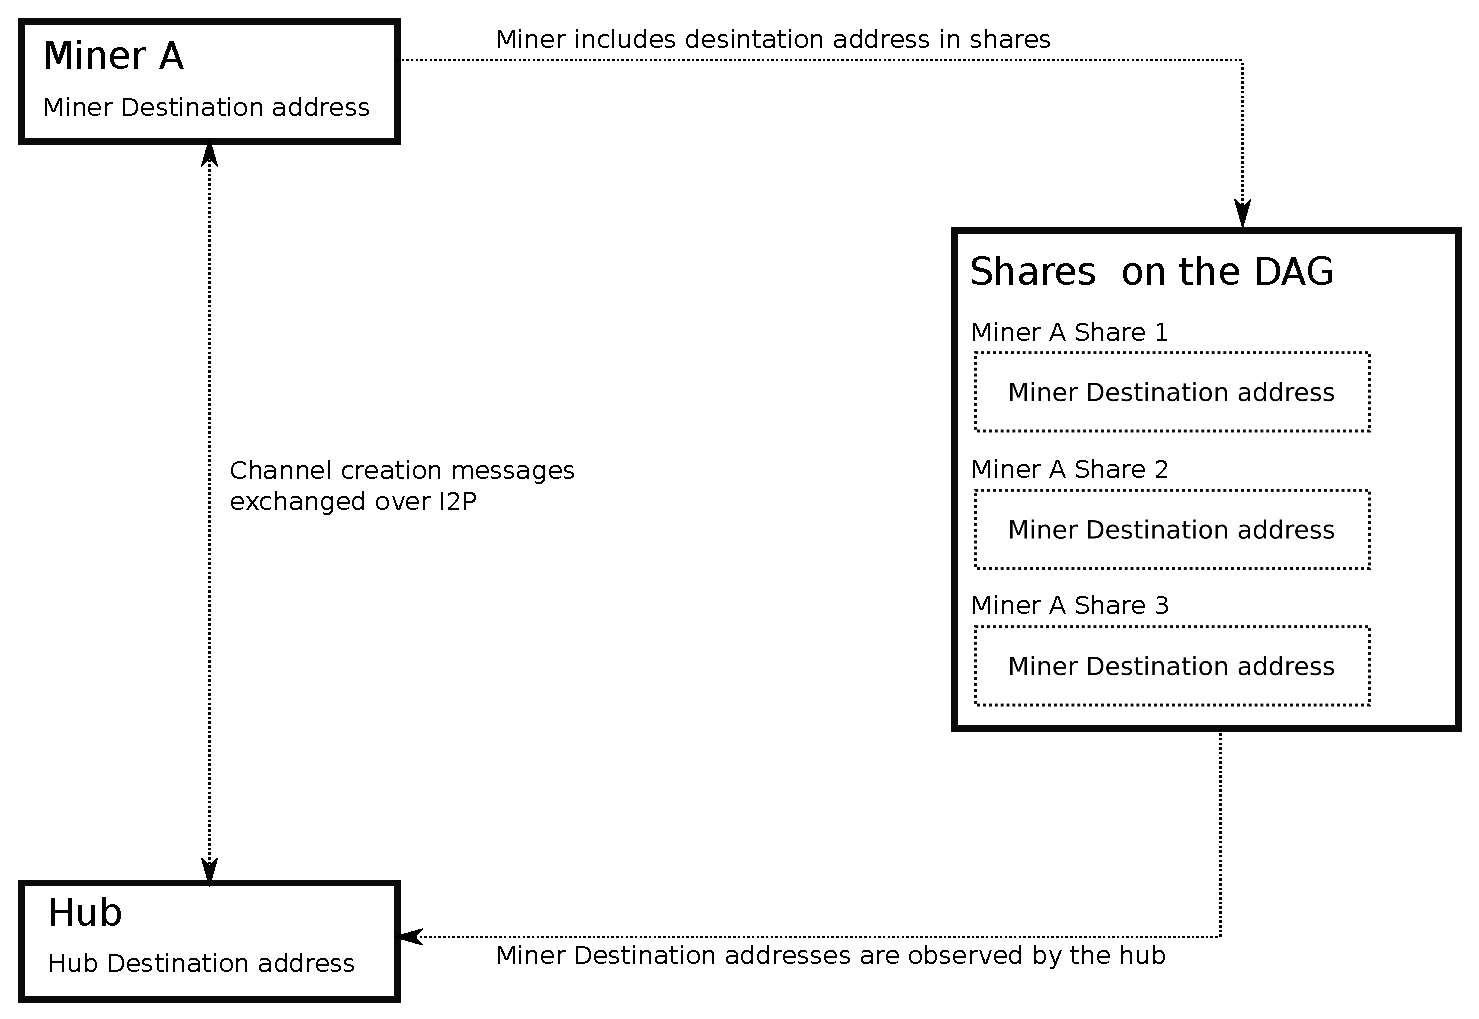
\includegraphics[width=0.75\textwidth]{new-miner-communication.eps}
    \caption{Discovery of miner I2P destination addresses enables
      communication for creating channels.}\label{fig:new-miner-communication}
  \end{center}
\end{figure}

\begin{figure}
  \begin{center}
    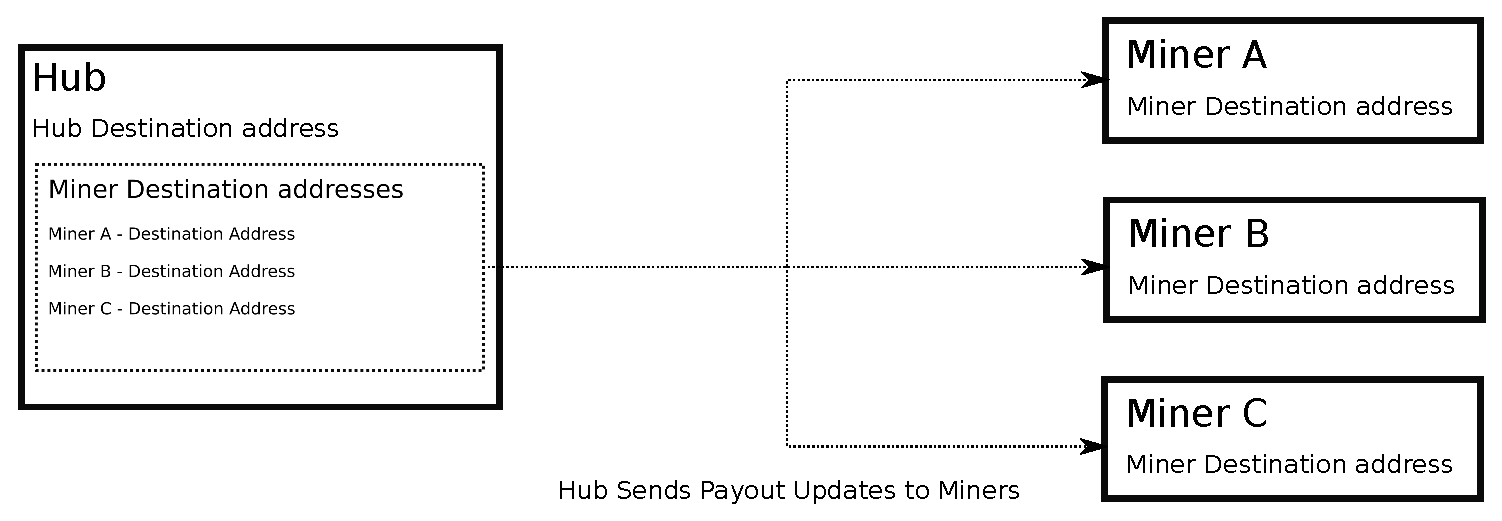
\includegraphics[width=0.8\textwidth]{payout-communication.eps}
    \caption{Hub sends one way updates to miners without revealing its
      destination address.}\label{fig:new-miner-communication}
  \end{center}
\end{figure}

There are two types of control messages exchanged between the hub and
the miner: 
\begin{enumerate*}
\item the channel creation messages when the miner first joins the
  pool and
\item the payout messages whenever a block is found.
\end{enumerate*}

Miners will run an I2P node next to their mining controller and setup
an incoming tunnel. Once the tunnel is ready, miners include their I2P
destination address in their share headers. The hub can then send
messages to the miner through the I2P tunnel.

The hub participates in the shares broadcast p2p network and
identifies a new miner along with the new miner's destination
address. Once the miner has mined for a certain time period, the hub
contacts the miner and provides its own destination address in the
message~\cite{i2p-streaming-library}. Figure~\ref{fig:new-miner-communication}
shows how the ``Miner A'' announces its I2P destination address,
enabling the hub to contact the miner for exchanging channel creation
messages. The hub in turn uses different destination addresses when
contacting each miner, further strengthening its anonymity and
resistance to DDoS attacks.

To prevent the tunnel endpoint and gateway from seeing the messages
being exchanged, the hub and the miner use I2P's layered encryption,
called garlic routing~\cite{i2p-garlic-routing}. With the destination
addresses of both the new miner and the hub known to each other the
two can proceed to anonymously setup a payment channel as described in
Section~\ref{ref:channels}.

To send payouts as channel state updates, the hub again uses the I2P
destination address of each miner and sends a one way message, with no
reply destination included in the message. This allows the hub to
remain anonymous and makes it relatively hard to DDoS the hub. The hub
sends all miners the updates to all payment channels. This allows the
miner who discovered a block to verify that the hub has paid everyone.

\section{Future Work}

Our proposal presents an approach to enable decentralised mining for
bitcoin. Apart from the work of describing the various components in
detail, we also want to provide results from simulations, formalised
proofs of rewards schemes and possible extensions to using multiple
hubs.

Before we work on implementing the system, our next step is to
simulate p2p mining network using ns-3~\cite{ns3} and make informed
decisions about how large a network a single hub can support. The
observations we want to make are how large a p2p network can be
sustained without an increase in work lost by miners. Each instance of
the pool uses a single hub and the p2p network of miners can grow as
long as miners are communicate \textsc{work} and \textsc{share}s with
each other within bounded latencies. We want to find the bounds of
these limits using a simulation.

We also want to specify the p2p protocols and the message formats for
both the \textsc{share}s propagation and channel management
networks. By publishing the specifications separate from the source
code, we aim to receive more feedback from the community. We want to
use the model presented in~\cite{incentives-compatible} to provide
proofs for how the rewards distribution is incentives compatible. We
would like to build further on the multiple hubs construction
described by Belcher once Taproot is activated on bitcoin.

\section{Acknowledgements}

Please to review! Many wow! ;)

\bibliography{proposal} 
\bibliographystyle{acm}

\end{document}
